\section{Single Particle Motion}
\begin{frame}{Larmor Orbit}
    A charged particle gyrates in the plane that is perpendicular to the magnetic field lines. Its gyration radius is called Larmor radius,
    \begin{equation}
        \rho = \frac{mv_\perp}{eB}
        \label{eq:larmor-radius}
    \end{equation}
    where $v_\perp$ is the speed in the direction perpendicular to magnetic field B.

    The gyration frequency is called Larmor frequency or cyclotron frequency
    \begin{equation}
        \omega_c = \frac{eB}{m}
        \label{eq:cyclotron-frequency}
    \end{equation}
\end{frame}

\begin{frame}{Particle Motion along B}
    \begin{itemize}
        \item If B field is uniform and no E field along $\mathbf{B}$, then the particle is moving with constant velocity in the direction of $\mathbf{B}$.
        \item If B field is uniform and there is a non-zero component of E along $\mathbf{B}$, then the particle will experience a force $eE_\parallel$ along $\mathbf{B}$.
        \item If B field has gradient in the direction of $\mathbf{B}$ (assuming no E). Then the particle will experience a force $-\frac{\frac{1}{2}mv\perp^2}{B}\grad_\parallel B$.
    \end{itemize}
\end{frame}

\begin{frame}{Particle Drifts - $\mathbf{E\times B}$ Drift}
    \begin{equation}
        \mathbf{v}_{E\times B} = \frac{\mathbf{E\times B}}{B^2}
        \label{eq:e-cross-b-drift}
    \end{equation}
    \begin{figure}
        \centering
        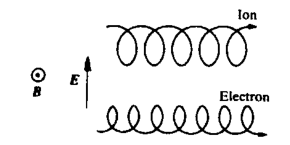
\includegraphics[width=0.7\textwidth]{figures/e-cross-b-drift.png}
        \caption{$\mathbf{E\times B}$ drift of ion and electron. $v_d=E/B$.}
        \label{fig:e-cross-b-drift}
    \end{figure}
\end{frame}

\begin{frame}{Particle Drifts - $\grad B$ Drift}
    \begin{equation}
        \mathbf{v}_{\grad B} = \text{sign}(e)\frac{1}{2}\rho\frac{\mathbf{B}\times\grad B}{B^2}v_\perp
        \label{eq:grad-b-drift}
    \end{equation}
    where $\text{sign}(e)$ is the sign of particle charge.
    \begin{figure}
        \centering
        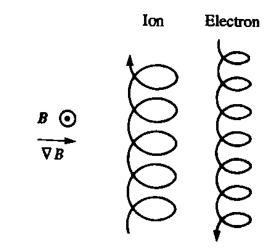
\includegraphics[width=0.4\textwidth]{figures/grad-b-drift.png}
        \caption{A gradient of B perpendicular to B gives ion and electron drifts in opposite directions.}
        \label{fig:grad-b-drift}
    \end{figure}
\end{frame}

\begin{frame}{Particle Drifts - Curvature Drift}
    \begin{equation}
        \mathbf{v}_{\grad B} = \frac{v_\parallel^2 + \frac{1}{2}v_\perp^2}{\omega_c}\frac{\mathbf{B}\times\grad B}{B^2}
        \label{eq:curvature-drift}
    \end{equation}
    \begin{figure}
        \centering
        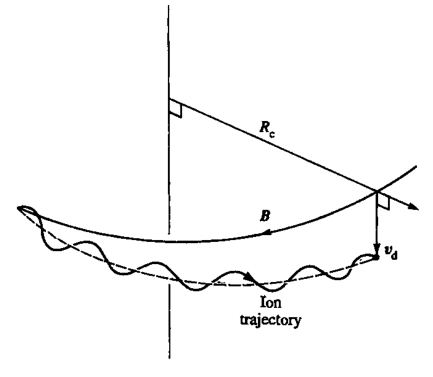
\includegraphics[width=0.5\textwidth]{figures/curvature-drift.png}
        \caption{Ion drift due to magnetic field curvature. Electrons drift in the opposite directions.}
        \label{fig:}
    \end{figure}
\end{frame}

\begin{frame}{Particle Drifts - Polarization Drift}
    \begin{equation}
        \mathbf{v}_{\grad B} = \frac{1}{\omega_cB}\dv{\mathbf{E}}{t}
        \label{eq:polarization-drift}
    \end{equation}
    \begin{figure}
        \centering
        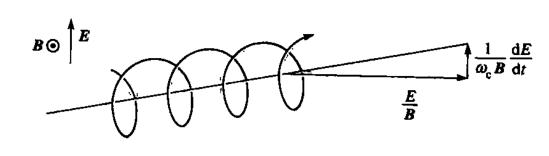
\includegraphics[width=0.7\textwidth]{figures/polarization-drift.png}
        \caption{Polarization drift of an ion caused by an increasing electric field perpendicular to the magnetic field. The electron drifts is in the opposite direction.}
        \label{fig:polarization-drift}
    \end{figure}
\end{frame}

\begin{frame}{Adiabatic Invariants}
    \begin{itemize}
        \item First adiabatic invariant: The magnetic moment, $\mu = \frac{\frac{1}{2}mv_\perp^2}{B}$, is constant if $\mathbf{B}$ changes very slowly.
        \item Second adiabatic invariant: This invariant $J$ is constant when the particle has a larger scale periodic motion. And $J = \oint v_\parallel\dd{l}$ where $\dd{l} = \mathbf{b}\cdot\dd{\mathbf{x}}$, $\mathbf{b}$ is the unit vector along $\mathbf{B}$.
        \item Third adiabatic invariant: If the periodic motion involved $J$ is subject to a drift and results in a larger scale periodic motion, then $J_3=\int v_d\dd{l}$ is invariant.
    \end{itemize}
\end{frame}